\phantomsection
\chapter[Analyzing the Coronavirus Spike Protein]{Analyzing the Coronavirus Spike Protein\chapsubhead{Chris Lee and Phillip Compeau}}
\label{chapter:coronavirus}
\renewcommand{\chaptertitle}{Analyzing the Coronavirus Spike Protein}
\addcontentsline{cc}{chapter}{Chapter \thechapter} % Adds chapter number to table of contents


\FloatBarrier

\section{A Tale of Two Doctors}
\label{sec:introduction}
\phantomsection

\begin{displayquote}
	One of the world's most important warning systems for a deadly new outbreak is a doctor's or nurse's recognition that some new disease is emerging and then sounding the alarm. It takes intelligence and courage to step up and say something like that, even in the best of circumstances.
	
	Tom Inglesby, Director of the Center for Health Security at Johns Hopkins Bloomberg School of Public Health
\end{displayquote}

\phantomsection
\subsection{The world's fastest outbreak}

On February 21, 2003, a Chinese doctor named Liu Jianlun flew to Hong Kong to attend a wedding and checked into Room 911 of the Metropole Hotel. The next day, he became too ill to attend the wedding and was admitted to a hospital. Two weeks later, Dr. Liu was dead.

On his deathbed, Dr. Liu stated that he had recently treated sick patients in Guangdong Province, China, where a highly contagious respiratory illness had infected hundreds of people. The Chinese government had made brief mention of this incident to the World Health Organization but had concluded that the likely culprit was a common bacterial infection. By the time anyone realized the severity of the disease, it was already too late to stop the outbreak. On February 23, a man who had stayed across the hall from Dr. Liu at the Metropole traveled to Hanoi and died after infecting 80 people. On February 26, a woman checked out of the Metropole, traveled back to Toronto, and died after initiating an outbreak there. On March 1, a third guest was admitted to a hospital in Singapore, where sixteen additional cases of the illness arose within two weeks.

Consider that it took four years for the Black Death, which killed over a third of all Europeans in the 14th Century, to travel from Constantinople to Kiev. Or that HIV took two decades to circle the globe. In contrast, this mysterious new disease had crossed the Pacific Ocean within a week of entering Hong Kong.

As health officials braced for the impact of the fastest-traveling virus in human history, panic set in. Businesses were closed, sick passengers were removed from airplanes, and Chinese officials threatened to execute anyone deliberately spreading the disease. In the process, the mysterious new illness earned a name: \textdef{Severe Acute Respiratory Syndrome}{Severe Acute Respiratory Syndrome}{FILL IN}, or \textdef{SARS}{SARS}{FILL IN}.

\phantomsection
\subsection{Finding the source of the outbreak}

SARS was deadly, killing close to 10% of those who became sick.[^cdc-factsheet] But it also struggled to spread within the human population, and it was contained in July 2003 with fewer than 10,000 confirmed symptomatic cases worldwide.

Scientists initially thought that humans had contracted SARS from palm civets, which are native to Guangdong. But research would later show that the disease likely originated in bats, a notorious disease carrier.

In 2017, researchers published the result of five years of sampling horseshoe bats from a cave in Yunnan province. They found that the bats harbored coronaviruses with remarkable genetic similarity to SARS, and they hypothesized that the virus may have come from horseshoe bats. Yet their work has become infamous because they identified additional viruses in the bats that were related to SARS but just as capable of entering human cells. Their words are now chilling:

\begin{displayquote}
	We have also revealed that various [viruses] ... are still circulating among bats in this region. Thus, the risk of spillover into people and emergence of a disease similar to SARS is possible. This is particularly important given that the nearest village to the bat cave we surveyed is only 1.1 km away, which indicates a potential risk of exposure to bats for the local residents. Thus, we propose that monitoring of SARSr-CoV evolution at this and other sites should continue, as well as examination of human behavioral risk for infection and serological surveys of people, to determine if spillover is already occurring at these sites and to design intervention strategies to avoid future disease emergence.
\end{displayquote}

\phantomsection
\subsection{A new threat emerges}

On December 30, 2019, a Chinese ophthalmologist named Li Wenliang sent a WeChat message to fellow doctors at Wuhan Central Hospital, warning them that he had seen several patients with symptoms resembling SARS. He urged his colleagues to wear protective clothing and masks to shield them from this new potential threat.

The next day, a screenshot of his post was leaked online, and local police summoned Dr. Li and forced him to sign a statement that he had "severely disturbed public order". He then returned to work, treating patients in the same Wuhan hospital.

Meanwhile, the World Health Organization (WHO) received reports of multiple pneumonia cases from the Wuhan Municipal Health Commission and activated a support team to assess the new disease. The WHO declared on January 14 that local authorities had seen "no clear evidence of human-to-human transmission of the novel coronavirus". By this point, it was now too late.

Throughout January, the virus silently raged through China, spreading to both South Korea and the United States as Lunar New Year celebrations took place within the country. By the end of the month, the disease was in 19 countries, becoming a pandemic and earning a name in the process: \textdef{coronavirus disease 2019 (COVID-19)}{coronavirus disease 2019 (COVID-19)}{FILL IN}.

As for Dr. Li? Despite warning against the risk of this new virus, he contracted the disease from one of his patients on January 8. He continued working in the hospital, and entered the hospital on January 31. Within a week, he was dead, one of the first of millions of COVID-19 casualties.

\phantomsection
\subsection{Why were the two outbreaks so different?}

The similarity between SARS and COVID-19 extends well beyond their symptoms. The respective viruses causing these diseases, \textdef{SARS coronavirus (SARS-CoV)}{SARS coronavirus (SARS-CoV)}{FILL IN} and \textdef{SARS coronavirus 2 (SARS-CoV-2)}{SARS coronavirus 2 (SARS-CoV-2)}{FILL IN} are both \textdef{coronaviruses}{coronaviruses}{FILL IN}, which means that their outer membranes are covered in a layer of \textdef{spike proteins}{spike proteins}{FILL IN} that cause them to look like the sun's corona during an eclipse.

\begin{figure}[h]
	\centering
	\mySfFamily
	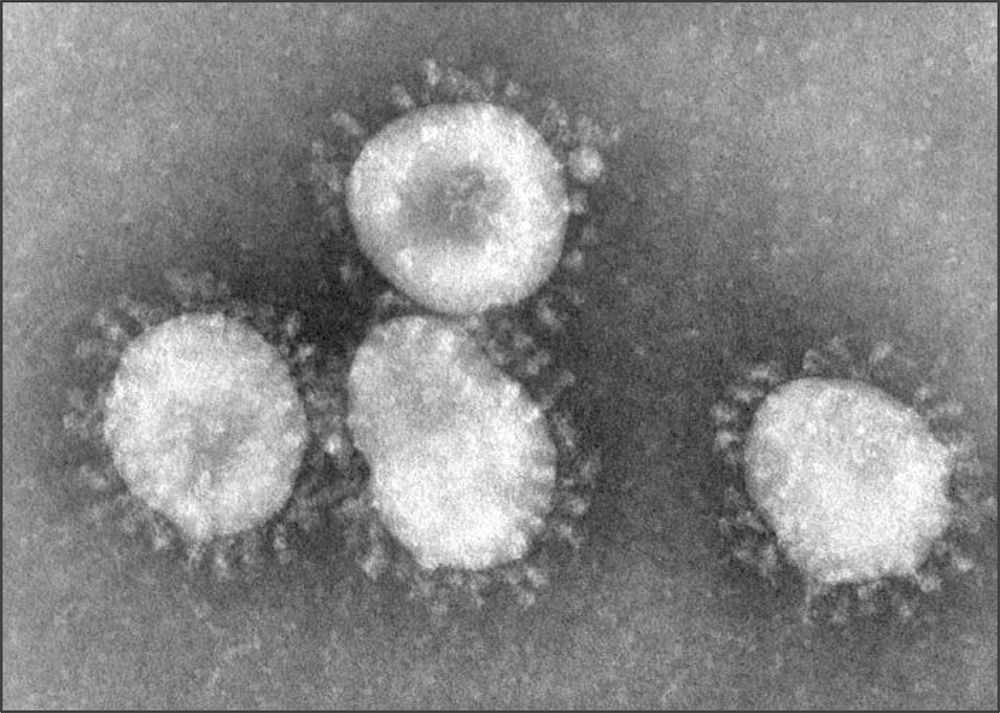
\includegraphics[width = 0.7\textwidth]{../images/coronavirus.png}
	\caption{Coronviruses as seen under a microscope. The fuzzy blobs on the cell surface are spike proteins, which the virus uses to gain entry to host cells. Figure courtesy F. Murphy and S. Whitfield, CDC.}
	\label{fig:coronavirus}
\end{figure}

Under a microscope, the two viruses look identical, and they use the same mechanism to infect human cells, when the spike protein on the virus surface bonds to the ACE2 enzyme on a human cell's membrane. So why did SARS fizzle, but SARS-CoV-2, a disease that is on average less harmful and less deadly to individuals who contract it, transform into a pandemic? The most likely explanation for the ability of SARS-CoV-2 to spread across far more countries and remain a public health threat even in the face of lockdowns is that it spreads more easily; that is, it is more \textdef{infectious}{infectious}{FILL IN}.

Part of the reason for the rapid spread of SARS-CoV-2 is that it can be spread by individuals that are asymptomatic, a method of transmission that was never found for SARS-CoV. But we also wonder if we can find a molecular explanation for the increased infectiousness of SARS-CoV-2.

In this chapter, we will place ourselves in the shoes of early SARS-CoV-2 researchers studying the new virus in January 2020. The virus's \textdef{genome}{genome}{FILL IN} (the 30,000 nucleotide sequence making up its DNA) was published on January 10, and an annotation of this genome showing the position of the virus's genes is shown in \autoref{fig:SARSCoV2Annotation}. Upon sequence comparison, SARS-CoV-2 was found to be related to several coronaviruses isolated from bats and distantly related to SARS-CoV.

\begin{figure}[h]
	\centering
	\mySfFamily
	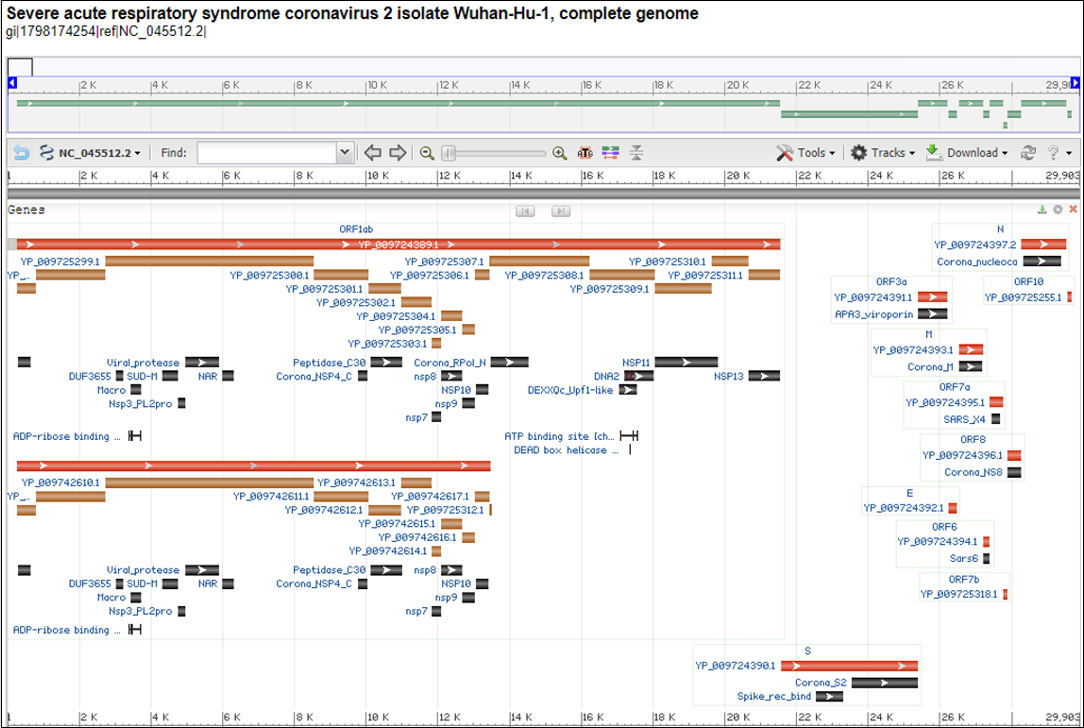
\includegraphics[width = 0.7\textwidth]{../images/SARSCoV2Annotation.png}
	\caption{An annotated genome of SARS-CoV-2. The Spike protein, found at the bottom of this image, is labeled "S" and begins at position 21,563. Accessed from GenBank: \url{https://go.usa.gov/xfzMM}}
	\label{fig:SARSCoV2Annotation}
\end{figure}

Recall from our discussion of transcription factors in \autoref{chapter:motifs} that by the central dogma of molecular biology, DNA is transcribed into RNA, which is then translated into protein. According to the genetic code, triplets of RNA nucleotides called codons are converted into single amino acids. The resulting chain of amino acids is called a \textdef{polypeptide}{polypeptide}{FILL IN}.

The polypeptide chain for the SARS-CoV-2 spike protein is shown below. Each of 20 possible amino acids is represented by a letter taken from the Latin alphabet (all letters except for "B", "J", "O", "U", "X", and "Z" are used for amino acids). Consider how such a global mayhem can ultimately be caused by something so tiny.

\texttt{>YP_009724390.1 S [organism=Severe acute respiratory syndrome coronavirus 2] [GeneID=43740568] \\
	MFVFLVLLPLVSSQCVNLTTRTQLPPAYTNSFTRGVYYPDKVFRSSVLHSTQDLFLPFFSNVTWFHAIHV
	SGTNGTKRFDNPVLPFNDGVYFASTEKSNIIRGWIFGTTLDSKTQSLLIVNNATNVVIKVCEFQFCNDPF
	LGVYYHKNNKSWMESEFRVYSSANNCTFEYVSQPFLMDLEGKQGNFKNLREFVFKNIDGYFKIYSKHTPI
	NLVRDLPQGFSALEPLVDLPIGINITRFQTLLALHRSYLTPGDSSSGWTAGAAAYYVGYLQPRTFLLKYN
	ENGTITDAVDCALDPLSETKCTLKSFTVEKGIYQTSNFRVQPTESIVRFPNITNLCPFGEVFNATRFASV
	YAWNRKRISNCVADYSVLYNSASFSTFKCYGVSPTKLNDLCFTNVYADSFVIRGDEVRQIAPGQTGKIAD
	YNYKLPDDFTGCVIAWNSNNLDSKVGGNYNYLYRLFRKSNLKPFERDISTEIYQAGSTPCNGVEGFNCYF
	PLQSYGFQPTNGVGYQPYRVVVLSFELLHAPATVCGPKKSTNLVKNKCVNFNFNGLTGTGVLTESNKKFL
	PFQQFGRDIADTTDAVRDPQTLEILDITPCSFGGVSVITPGTNTSNQVAVLYQDVNCTEVPVAIHADQLT
	PTWRVYSTGSNVFQTRAGCLIGAEHVNNSYECDIPIGAGICASYQTQTNSPRRARSVASQSIIAYTMSLG
	AENSVAYSNNSIAIPTNFTISVTTEILPVSMTKTSVDCTMYICGDSTECSNLLLQYGSFCTQLNRALTGI
	AVEQDKNTQEVFAQVKQIYKTPPIKDFGGFNFSQILPDPSKPSKRSFIEDLLFNKVTLADAGFIKQYGDC
	LGDIAARDLICAQKFNGLTVLPPLLTDEMIAQYTSALLAGTITSGWTFGAGAALQIPFAMQMAYRFNGIG
	VTQNVLYENQKLIANQFNSAIGKIQDSLSSTASALGKLQDVVNQNAQALNTLVKQLSSNFGAISSVLNDI
	LSRLDKVEAEVQIDRLITGRLQSLQTYVTQQLIRAAEIRASANLAATKMSECVLGQSKRVDFCGKGYHLM
	SFPQSAPHGVVFLHVTYVPAQEKNFTTAPAICHDGKAHFPREGVFVSNGTHWFVTQRNFYEPQIITTDNT
	FVSGNCDVVIGIVNNTVYDPLQPELDSFKEELDKYFKNHTSPDVDLGDISGINASVVNIQKEIDRLNEVA
	KNLNESLIDLQELGKYEQYIKWPWYIWLGFIAGLIAIVMVTIMLCCMTSCCSCLKGCCSCGSCCKFDEDD
	SEPVLKGVKLHYT}

We will ask ourselves two questions. First, can we use this sequence of amino acids to determine the structure of its spike protein? Second, once we know the structure of the SARS-CoV-2 spike protein, how does its structure and function differ from the same protein in SARS-CoV?

We will split our work on these questions over two parts. If you are already familiar with protein structure prediction, then you may want to skip ahead to the second part of the chapter, in which we discuss differences between the spike proteins of the two viruses.

\FloatBarrier
\phantomsection

\section{Protein Structure Prediction is Difficult}
\label{sec:structure_intro}
\phantomsection
\subsection{Determining protein structure is fundamental to understanding protein function}

In the \autoref{sec:introduction}, we showed the polypeptide chain for the SARS-CoV-2 spike protein. After this polypeptide chain is formed, it will "fold" into a three-dimensional shape and attach to the exterior of the virus. The folding process occurs spontaneously and without any outside influence, and the same polypeptide chain will almost always fold into the same 3-D structure in a manner of microseconds. This means that nature is applying some "magic algorithm" that produces the folded structure of a protein from its sequence of amino acids. But how does this algorithm work?

Predicting the folded structure of a polypeptide is called the \textdef{structure prediction problem}{structure prediction problem}{FILL IN}, and this problem is simple to state but deceptively difficult to solve. In fact, it has been an active area of biological research for several decades.

Why do we care about protein structure? Knowing a protein's structure is essential to determining its function and how it interacts with other proteins or molecules in its environment. Determining protein function is still an active area of research: there are still a few thousand proteins in humans alone whose function is unknown.

Furthermore,  a huge amount of biological research is devoted to understanding protein interactions. For example, a disease may be caused by a faulty protein, in which case researchers want to find a drug that binds to the protein and causes some change of interest in that protein, such as inhibiting its behavior.

For a more visual example of how protein structure affects protein function, consider the following video of a ribosome (which is a complex of RNA and proteins) translating a messenger RNA into protein. For translation to succeed, the ribosome needs to have a very precise shape, including a "slot" into which the messenger RNA strand can fit.

\texttt{mRNA Translation (Youtube video)} \\
% include video id="TfYf_rPWUdY" provider="youtube" %

As we have seen throughout this course, molecular interactions are ruled by probability. Any two molecules may \textit{interact}, but their rate of \textit{dissociation} will be much higher if they do not fit together well. Furthermore, two colliding molecules need to have the correct orientation in order to produce an interaction

Because structure prediction is such a fundamental problem, researchers wish to catalog the varied shapes of different proteins. This variety is evident in \autoref{fig:different_protein_shapes_2020}, which shows the "proteins of the month" in 2020 named by the \textdef{Protein Data Bank (PDB)}{Protein Data Bank (PDB)}{FILL IN}. Yet the question remains: how do we know these protein structures?

\begin{figure}[h]
	\centering
	\mySfFamily
	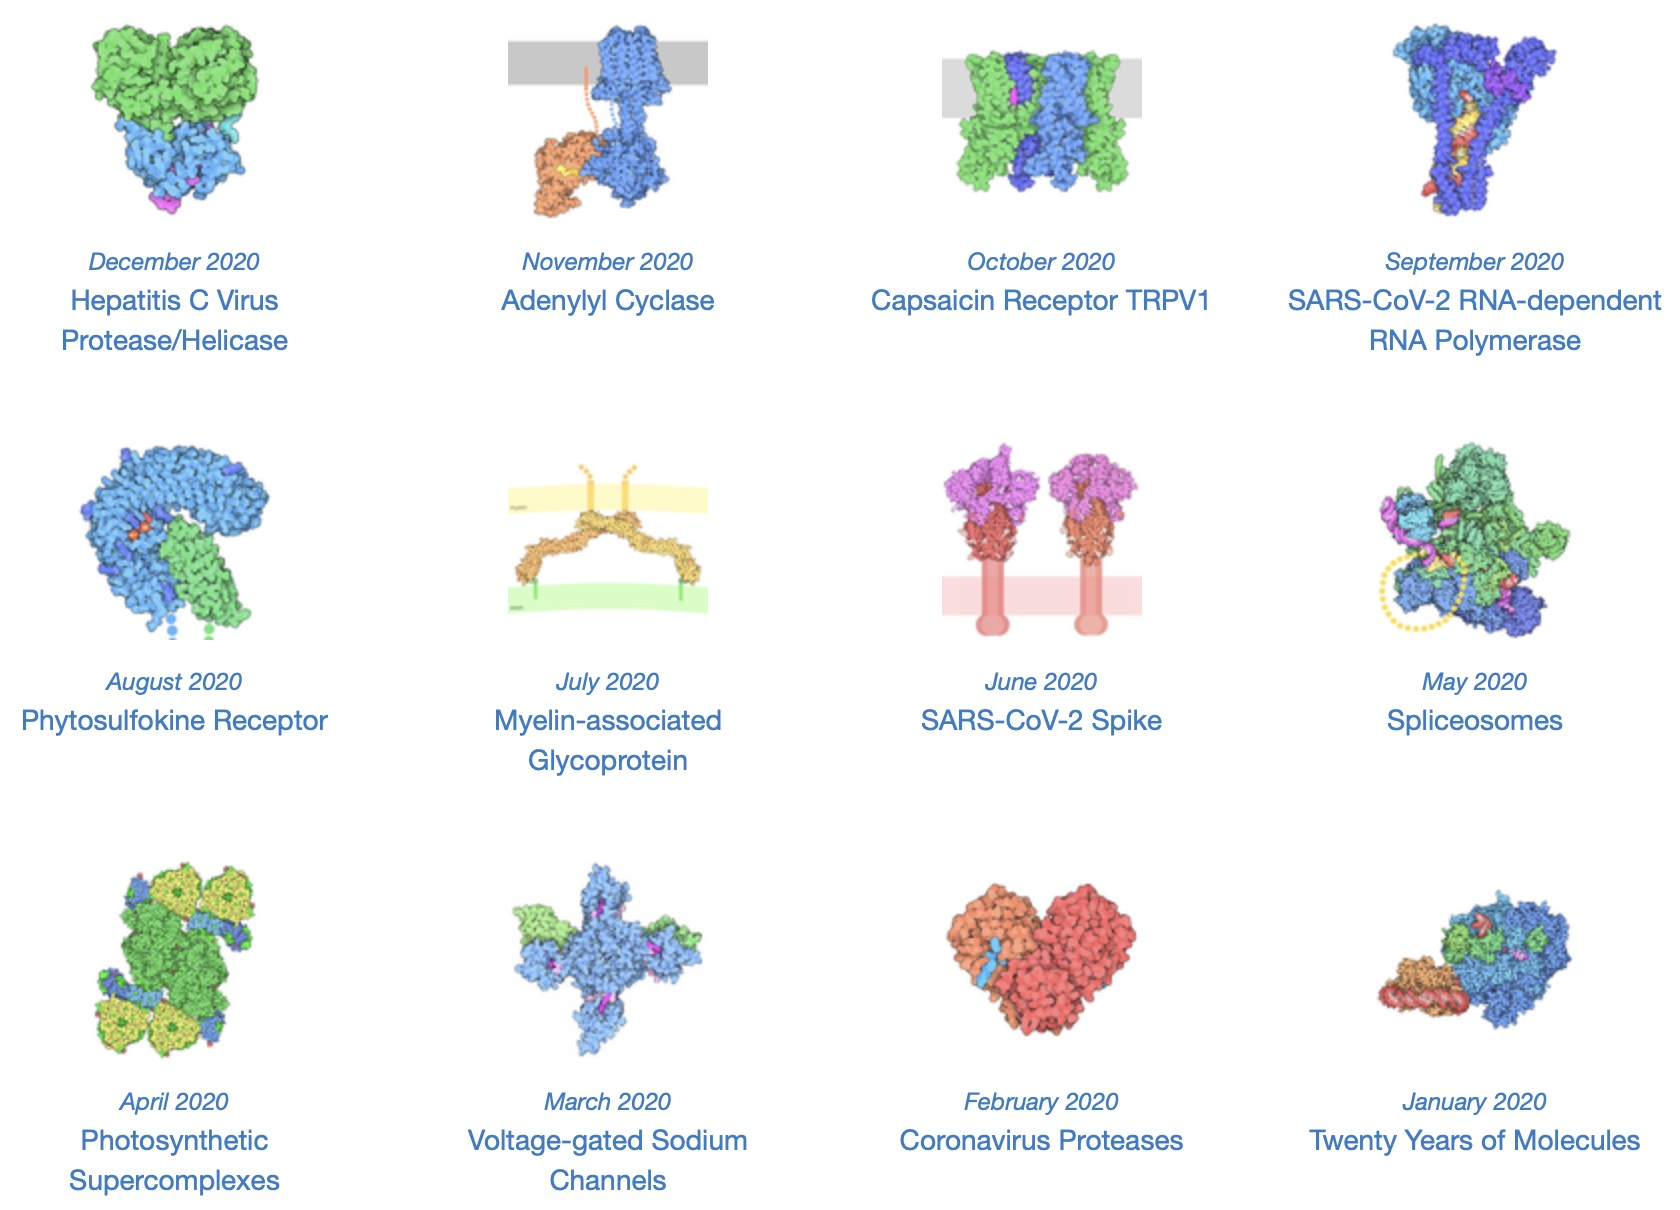
\includegraphics[width = 0.7\textwidth]{../images/different_protein_shapes_2020.jpg}
	\caption{Each "molecule of the month" in 2020 named by the PDB. These proteins have widely varying shapes and accomplish a wide variety of cellular tasks. Note that the SARS-CoV-2 spike protein was the molecule of the month in June 2020. Image courtesy: David Goodsell.}
	\label{fig:different_protein_shapes_2020}
\end{figure}

\phantomsection
\subsection{Laboratory methods for determining protein structure}

We will introduce two popular and sophisticated laboratory methods for accurately determining protein structure. We appeal to high-quality videos explaining them if you are interested.

In \textdef{X-ray crystallography}{X-ray crystallography}{FILL IN}, researchers crystallize many copies of a protein and then shine an intense beam of X-rays at the crystal. The light hitting the protein is diffracted, creating patterns from which the position of every atom in the protein can be inferred. If you are interested in learning more about X-ray crystallography, check out the following excellent two-part video series from The Royal Institution.

\texttt{Understanding Crystallography Part 1 (Youtube video)} \\
% include video id="gLsC4wlrR2A" provider="youtube" %

\texttt{Understanding Crystallography Part 1 (Youtube video)} \\
% include video id="WJKvDUo3KRk" provider="youtube" %

X-ray crystallography is over a century old and has been the \textit{de facto} approach for protein structure determination for decades. Yet a newer method is now rapidly replacing X-ray crystallography.

In \textdef{cryo-electron microscopy (cryo-EM)}{cryo-electron microscopy (cryo-EM)}{FILL IN}, researchers preserve thousands of copies of a protein in non-crystalline ice and then examine these copies with an electron microscope. Check out the following YouTube video from the University of California San Francisco for a detailed discussion of cryo-EM.

\texttt{What is Cryo-Electron Microscopy (Youtube video)} \\
% include video id="WJKvDUo3KRk" provider="youtube" %

Unfortunately, laboratory approaches for structure determination are expensive and cannot be used on all proteins. X-ray crystallography costs upward of \$2,000 per protein; furthermore, crystallizing a protein is a challenging task, and each copy of the protein must line up in the same way, which does not work for very flexible proteins. As for cryo-EM, an electron microscope costs upwards of millions of dollars. And to study bacterial proteins, we need to culture the bacteria in the lab, but microbiologists have estimated that less than 2\% of bacteria can currently be cultured.

Protein structures that have been determined experimentally are typically stored in the PDB. This database contains over 160,000 proteins, most of which have been added this century.

This number may seem large, but a recent study estimated that humans have between 620,000 and 6.13 million protein isoforms (i.e., differently-shaped protein variants). If we hope to catalog the proteins of all living things, then our work on structure determination is just beginning.

\phantomsection
\subsection{What makes protein structure prediction so difficult?}

Predicting protein structure from amino acid sequence is very challenging. On the one hand, small perturbations in the sequence of a protein can drastically change the protein's shape and even render it useless. On the other, different amino acids can have similar chemical properties, and so some mutations will hardly change the shape of the protein. As a result, two very different amino acid sequences can fold into proteins with similar structure and comparable function.

For example, \autoref{fig:SequenceStructureExample} compares the sequences and structures of hemoglobin subunit alpha taken from three species: humans (PDB: 1si4), shortfin mako sharks (PDB: 3mkb), and emus (PDB: 3wtg). Hemoglobin is the oxygen-transport protein in the blood, consisting of two alpha "subunit" proteins and two beta subunit proteins that combine into a protein complex; because hemoglobin is well-studied and much shorter than the SARS-CoV-2 spike protein, we will use it as an example throughout this module. The alpha subunits for the three species are markedly different in terms of amino acid sequence, and yet their 3-D structures are essentially identical.

\begin{figure}[h]
	\centering
	\mySfFamily
	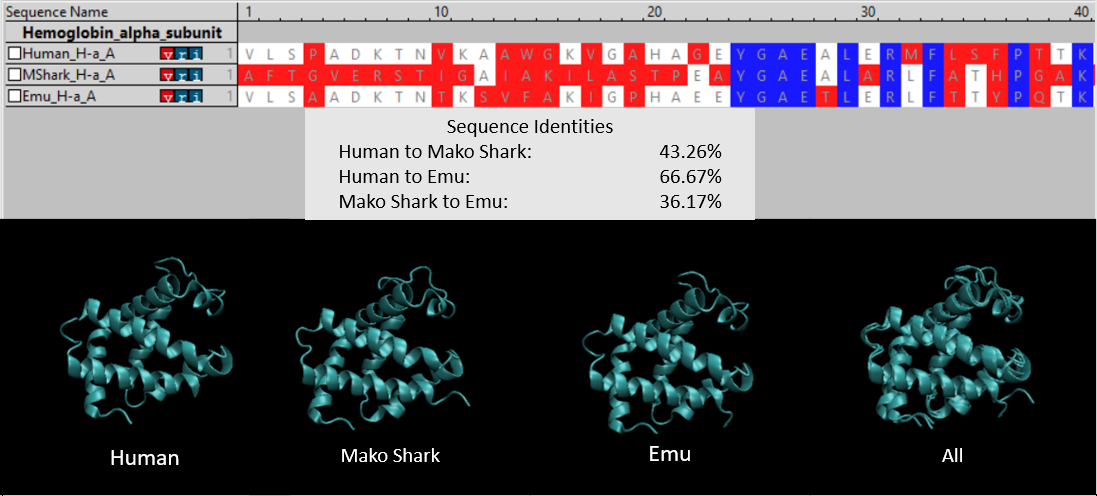
\includegraphics[width = 0.7\textwidth]{../images/SequenceStructureExample.png}
	\caption{(Top) An amino acid sequence comparison of the first 40 (out of 140) amino acids of hemoglobin subunit alpha for three species: human, shortfin mako shark, and emu. A column is colored blue if all three species have the same amino acid, white if two species have the same amino acid, and red if all amino acids are different. Sequence identity calculates the number of positions in two amino acid sequences that share the same amino acid. (Bottom) Side by side comparisons of the 3-D structures of the three proteins. The final figure on the right superimposes the first three structures to highlight their similarities.}
	\label{fig:SequenceStructureExample}
\end{figure}

Another reason why protein structure prediction is so difficult is because a polypeptide is very flexible, with the ability to rotate in multiple ways at each amino acid, which means that the polypeptide is able to fold into a staggering number of different shapes. A good analogy for polypeptide flexibility is the "Rubik's Twist" puzzle, shown in the video below, which consists of a linear chain of flexible blocks that can form a huge number of different shapes.

\texttt{Rubik's Snake animation (Youtube video)} \\
% include video id="auNLb75QRfg" provider="youtube" %

The flexibility of a polypeptide owes to the molecular structure of amino acids. As shown in \autoref{fig:AminoAcid}, an amino acid comprises four parts. In the center, a carbon atom (called the \textdef{alpha carbon}{alpha carbon}{FILL IN}) is connected to four different molecules: a hydrogen atom (H), a \textdef{carboxyl group}{carboxyl group}{FILL IN} (–COOH), an \textdef{amino group}{amino group}{FILL IN} (-NH\textsubscript{2}), and a \textdef{side chain}{side chain}{FILL IN} (denoted "R" and often called an \textdef{R group}{R group}{FILL IN}). The side chain is a molecule that differs between different amino acids and ranges in mass from a single hydrogen atom (glycine) up to -C\textsubscript{8}H\textsubscript{7}N (tryptophan).

\begin{figure}[h]
	\centering
	\mySfFamily
	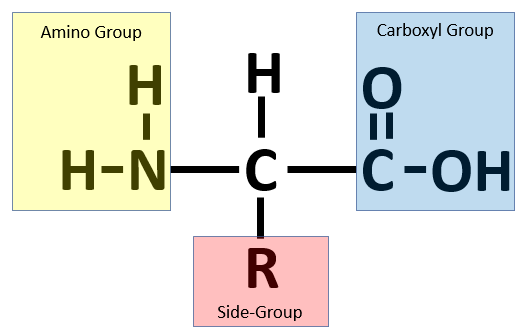
\includegraphics[width = 0.7\textwidth]{../images/AminoAcid.png}
	\caption{An amino acid consists of a central, alpha carbon attached to a hydrogen atom, a side group, a carboxyl group, and an amino group.}
	\label{fig:AminoAcid}
\end{figure}

To form a polypeptide chain, consecutive amino acids are linked together during a condensation reaction in which the amino group of one amino acid is joined to the carboxyl group of another, while a water molecule (H\textsubscript{2}O) is expelled (see in \autoref{fig:dipeptide_reaction}).

\begin{figure}[h]
	\centering
	\mySfFamily
	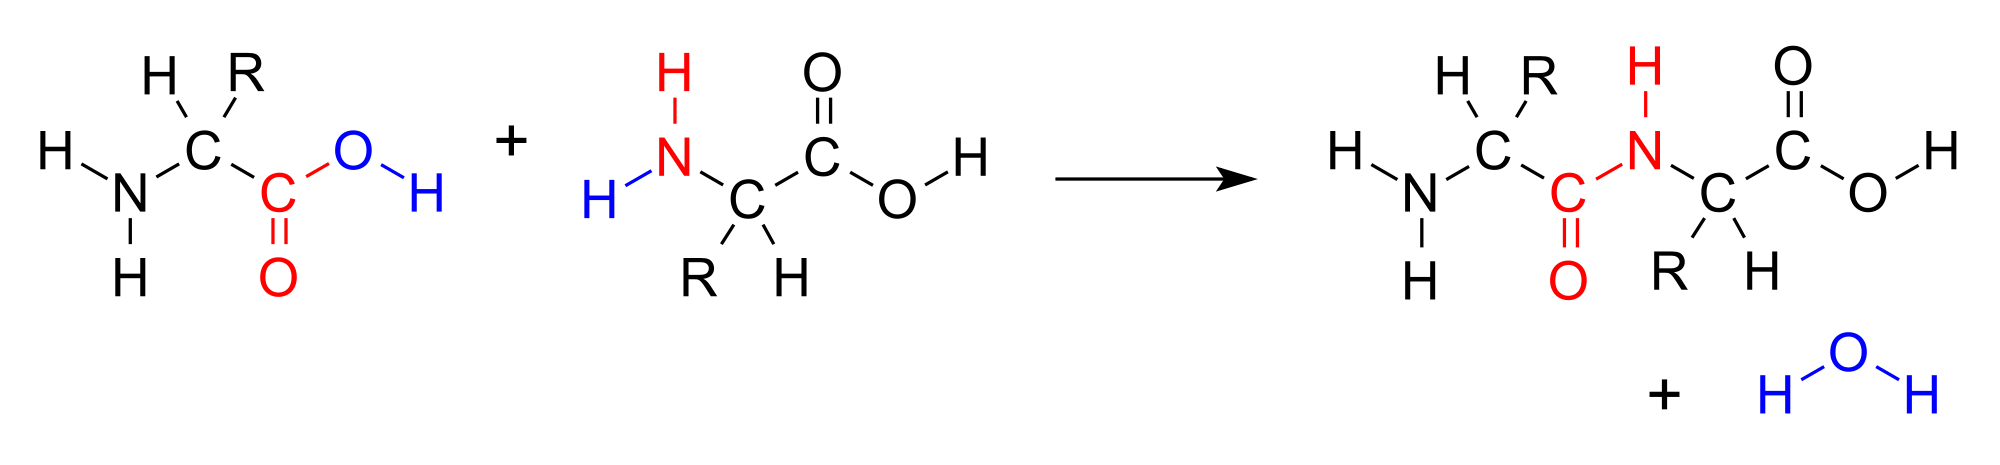
\includegraphics[width = 0.7\textwidth]{../images/dipeptide_reaction.png}
	\caption{A condensation reaction joins two amino acids into a "dipeptide" by joining the amino group of one amino acid to the carboxyl group of the other. A water molecule is expelled, which is why the reaction is a condensation reaction. Source: \url{https://bit.ly/3q0Ph8V}}
	\label{fig:dipeptide_reaction}
\end{figure}

The resulting bond that is produced between the carbon atom of one amino acid's carboxyl group and the nitrogen atom of the next amino acid's amino group, called a \textdef{peptide bond}{peptide bond}{FILL IN}, is very strong. The peptide has very little rotation around this bond, which is almost always locked at 180\textdegree. As peptide bonds are formed between adjacent amino acids, the polypeptide chain takes shape, as shown in the figure below.

\begin{figure}[h]
	\centering
	\mySfFamily
	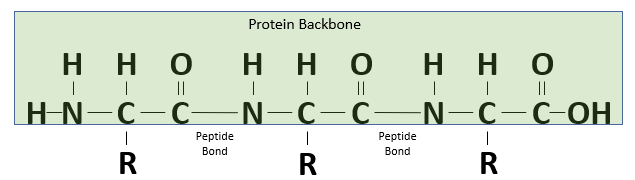
\includegraphics[width = 0.7\textwidth]{../images/Backbone.png}
	\caption{A protein backbone formed of three amino acids.}
	\label{fig:backbone}
\end{figure}

However, the bonds \textit{within} an amino acid, joining the alpha carbon to its carboxyl group and amino group, are not as rigid, and the polypeptide is free to rotate around these two bonds. This rotation produces two angles of interest, called the \textdef{phi angle (φ)}{phi angle (φ)}{FILL IN} and \textdef{phi angle (ψ)}{psi angle (ψ)}{FILL IN} (see \autoref{fig:torsion_angles}), which are formed at the alpha carbon's connections to its amino group and carboxyl group, respectively.

\begin{figure}[h]
	\centering
	\mySfFamily
	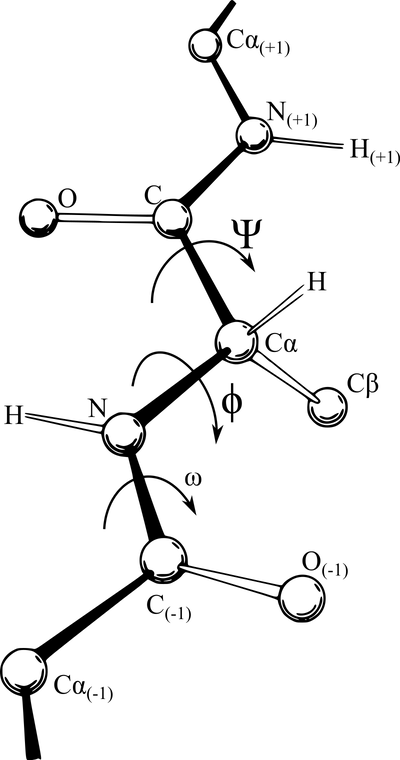
\includegraphics[width = 0.7\textwidth]{../images/torsion_angles.png}
	\caption{A polypeptide chain of multiple amino acids with the torsion angles φ and ψ indicated. The angle ω indicates the angle of the peptide bond, which is typically 180\textdegree. Image courtesy: Adam Rędzikowski.}
	\label{fig:torsion_angles}
\end{figure}

\url{https://youtu.be/1usemtIYe_s} is an excellent video from Jacob Elmer illustrating how changing φ and ψ at a single amino acid can drastically reorient a protein's shape.

A polypeptide with $$n$$ amino acids will have $$n - 1$$ peptide bonds, meaning that its shape is influenced by $$n - 1$$ phi angles and $$99 n - 1$$ psi angles. If each bond has $$k$$ stable conformations, then there are $$k^{2n-2}$$ total possible conformations of the polypeptide. For example, if $$k$$ is 3 and $$n$$ is just 100 (a short polypeptide), then the number of potential protein structures is more than the number of atoms in the universe! (The concept of combinatorial explosion, introduced in \autoref{chapter:chemotaxis}, appears again.) The ability for the protein to reliably find a single conformation using the magic algorithm despite such an enormous number of potential shapes is called \textdef{Levinthal's paradox}{Levinthal's paradox}{FILL IN}.

Although protein structure prediction is difficult, it is not impossible; nature's algorithm is not, after all, magic. Furthermore, researchers have spent decades cataloging the genomes of thousands of species. As a result, biologists know the \textit{sequence} of amino acids for many proteins whose structures have not been validated experimentally. In our case, although the SARS-CoV-2 genome was sequenced in January 2020, the structure of its spike protein was unknown at that time.  In the next lesson, we will place ourselves in the shoes of early SARS-CoV-2 researchers working before the structure of the virus's spike protein had been experimentally determined to see if we can predict its structure and give biologists a head start on fighting the pandemic.

